\PassOptionsToPackage{implicit=true}{hyperref}
\documentclass[10pt, aspectratio=169, compress, protectframetitle, handout]{beamer}
\usepackage[utf8]{inputenc}
\usepackage[english]{babel}
\usepackage{appendixnumberbeamer}
% handout to deactivate \uncover
% usetitleprogressbar might be needed
%\usepackage{beamerprosper}
\usepackage{comment}
% Load BEFORE the theme
\usepackage[normalem]{ulem}
\usepackage[T1]{fontenc}

\usetheme[progressbar=frametitle,block=fill,numbering=fraction]{metropolis}
\setbeamertemplate{blocks}[rounded][shadow=true]

% Change Colors/Width of Progress Bars 
\makeatletter
%\setlength{\metropolis@titleseparator@linewidth}{1pt}
\setlength{\metropolis@progressonsectionpage@linewidth}{0.8pt}
\setlength{\metropolis@progressinheadfoot@linewidth}{1pt}
\makeatother

%\setbeamertemplate{note page}[plain]
%\setsansfont[
%     Extension      = .otf,
%     UprightFont    = *-Light,
%     ItalicFont     = *-LightItalic,
%     BoldFont       = *-Regular,
%     BoldItalicFont = *-RegularItalic
% ]{FiraSans}
%\setmonofont[
%     Extension   = .otf,
%     UprightFont = *-Regular,
%     BoldFont    = *-Medium
%]{FiraMono}


\newcommand{\putbg}{\usebackgroundtemplate{
\includegraphics[width=\paperwidth,height=\paperheight]{background-vector_169}}}
\newcommand{\putbgdark}{\usebackgroundtemplate{
\includegraphics[width=\paperwidth,height=\paperheight]{background-vector-dark_169}}}


%%% Math
\usepackage{amsfonts}
\usepackage{amsthm}
\usepackage{amsmath}
\usepackage{amssymb}

%%% Algorithms
\usepackage{algorithm}
\usepackage{algcompatible}
\usepackage{algpseudocode}
\renewcommand{\Comment}[2][.34\linewidth]{%
  \leavevmode\hfill\makebox[#1][l]{$\triangleright$~#2}} % To align the comments
  
%%% Symbols
\newcommand{\uv}{\mathbf{u}}    % u vector
\newcommand{\ev}{\mathbf{e}}    % e vector
\newcommand{\vv}{\mathbf{v}}    % v vector
\newcommand{\NN}{\mathrm{NN}}
\def\globals{\mathbf{u}}

\usepackage[export]{adjustbox}
\usepackage[]{enumitem}
\usepackage{datetime}
\usepackage{textpos}
\usepackage{marvosym} % Smile
\usepackage{wrapfig} % To wrap figures wih text
\usepackage{cleveref} % To fix autoref links not working
% Fixes bad positioning of hats
\usefonttheme{professionalfonts}%[onlymath]{serif}
\PassOptionsToPackage{hyphens}{url}\usepackage{hyperref} % to break the links
\hypersetup{
    colorlinks=true,
    linkcolor=,      % color of internal links
    urlcolor=blue,   % color of external links
    citecolor=blue,  % color of links to bibliography
}


%%% Bibliografia
\usepackage[autostyle]{csquotes}
\usepackage[backend=biber]{biblatex}

% https://tex.stackexchange.com/questions/68080/beamer-bibliography-icon
\setbeamertemplate{bibliography item}{%
  \ifboolexpr{ test {\ifentrytype{book}} or test {\ifentrytype{mvbook}}
    or test {\ifentrytype{collection}} or test {\ifentrytype{mvcollection}}
    or test {\ifentrytype{reference}} or test {\ifentrytype{mvreference}} }
    {\setbeamertemplate{bibliography item}[book]}
    {\ifentrytype{online}
       {\setbeamertemplate{bibliography item}[online]}
       {\setbeamertemplate{bibliography item}[article]}}%
  \usebeamertemplate{bibliography item}}

\defbibenvironment{bibliography}
  {\list{}
     {\settowidth{\labelwidth}{\usebeamertemplate{bibliography item}}%
      \setlength{\leftmargin}{\labelwidth}%
      \setlength{\labelsep}{\biblabelsep}%
      \addtolength{\leftmargin}{\labelsep}%
      \setlength{\itemsep}{\bibitemsep}%
      \setlength{\parsep}{\bibparsep}}}
  {\endlist}
  {\item}

\addbibresource{biblio.bib}


%%% Metadati
\graphicspath{{figures/PNG/}{figures/PDF/}{figures/}}
\newdateformat{monthyear}{\monthname[\THEMONTH] \THEYEAR}
\title{\vspace*{1.5cm}An algorithmic reasoning approach to GNNs}
\subtitle{A project for the \emph{Deep Learning} course}
\author{Angela Carraro, Matteo Scorcia}
\date{}
\institute{\scshape DSSC + IN20 - UniTS
\vfill

\includegraphics[valign=c, height=0.7cm]{logo_dssc_alt}
\hspace*{0.5cm}

\includegraphics[valign=c, height=0.75cm]{Logo_units_blu}
}

\addtobeamertemplate{frametitle}{}{%
\begin{textblock*}{100mm}(0.90\textwidth,-0.94cm)
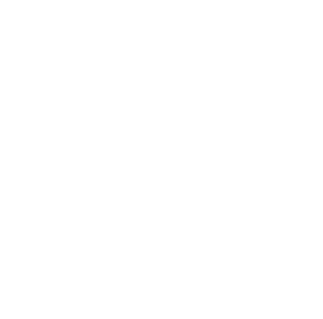
\includegraphics[valign=c, height=0.4cm]{logo_dssc_alt_white}
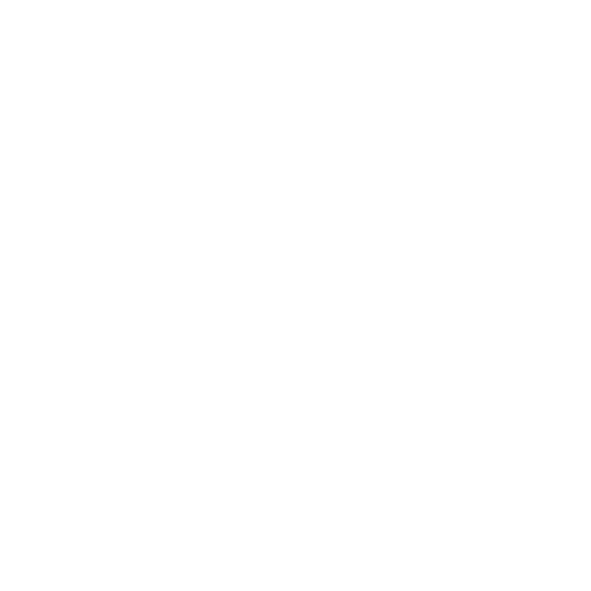
\includegraphics[valign=c, height=0.45cm]{Logo_units_white}
\end{textblock*}}

\begin{document}

{\putbg\maketitle}


%\begin{frame}{Contents}
%	\tableofcontents
%\end{frame}


\begin{frame}{Aim of the project}

    \alert{Graph Neural Networks} can have a lot of meanings, there isn't just one architecture that can be recognized as “GNN”. We will try to understand the general, abstract structure of a GNN that is presented in the book \cite{HamiltonGRLBook} (which also includes \cite{battaglia2018relational}) and to shed light about the relational inductive bias and combinatorial generalization of a GNN.
    
    Our motivation is to better understand the extent to which graph neural networks are capable of \textbf{precise and logical reasoning}.
    
    Our motivation is to better understand the extent to which graph neural networks are capable of \textbf{predict something, given a graph structured dataset}.
    
    Our goal is to understand why GNNs are needed and how it works in respect to a "classic" deep learning structure.
    
\end{frame}


{\putbg
\section{Graph Analysis}
}


\begin{frame}{Introduction}
    
    Graphs are a widespread data structure and a universal language for describing and modelling complex systems. In the most general view, a graph is simply a collection of objects (i.e., nodes), along with a set of interactions (i.e., edges) between pairs of these objects. 

    \begin{columns}[onlytextwidth]
        \begin{column}{.5\textwidth-.25cm}
            Graphs are an important building block since they can naturally encode an \alert{entity-relationship structure}, as well as an \alert{invariance to permutations} (of both nodes and edges) and awareness of \alert{input sparsity}.
        \end{column}
        \begin{column}{.5\textwidth-.25cm}
            \begin{figure}
                \centering
                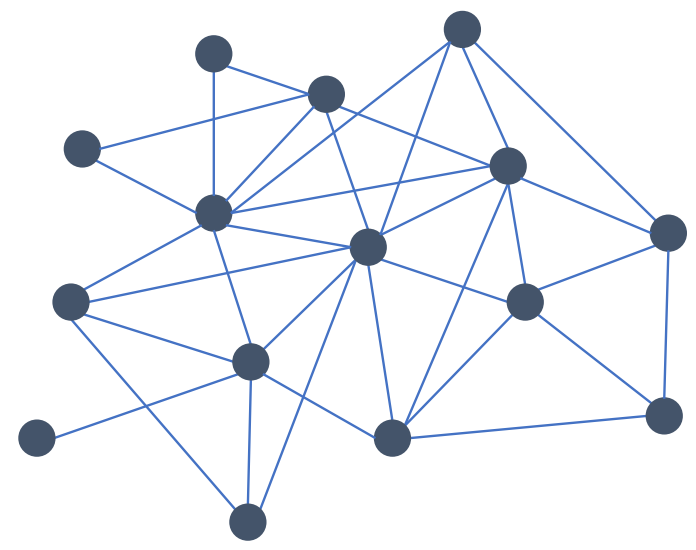
\includegraphics[width=3.8cm]{figures/Graph}
                \caption{A graph.}
            \end{figure}
        \end{column}
    \end{columns}
    
\end{frame}


\begin{frame}{Basics}
    
    \begin{block}{Definition}
        A \alert{graph} is a tuple $G = (V, E)$ where $V$ is the set of nodes and $E$ is the set of edges between these nodes. We denote an edge going from node $u \in V$ to node $v \in V$ as $(u, v) \in E$, so $E \subseteq V \times V$. The graph is \textbf{undirected} if $(u, v) \in E \Longleftrightarrow  (v, u) \in E$, otherwise it is \textbf{directed}.
    \end{block}
    
    Given a node $u$ in the graph, $\mathcal N(u)$ is $u$'s graph neighborhood.
    
    A convenient way to represent graphs is through an \alert{adjacency matrix} $\mathbf A \in \mathbb R^{|V| \times |V|}$, with $\mathbf A[u, v] = 1$ if $(u, v) \in E$ and $\mathbf A[u, v] = 0$ otherwise. If the graph is undirected the matrix in \emph{symmetric}. If the graph has weighted edges we have that $\mathbf A[u,v] \in \mathbb R$.
    
    We also have \alert{node-level attributes / features} represented using a matrix $\mathbf X \in \mathbb R^{d \times |V|}$ (with the ordering of the nodes consistent with the ordering in the adjacency matrix).
    
    In some cases we also have \alert{graph features}, which are real-valued \emph{features associated with entire graphs}.
    
\end{frame}


\begin{frame}{Machine learning on graphs}

    Machine learning tasks on graph data fall in one of these four categories:
    \begin{itemize}[topsep=4pt,itemsep=8pt]
        \item[{$\bullet$}] {\makebox[3.8cm][l]{\alert{\emph{node classification}}:} predict the label $y_u$ associated with all the nodes $u \in V$}\\
        \quad $\longrightarrow$ \; E.g., predicting whether a user is a bot in a social network
        
        \item[{$\bullet$}] {\makebox[3.8cm][l]{\alert{\emph{edge prediction}}:}
        infer the edges between nodes in a graph}\\ 
        %predict if there exists an edge between two nodes}\\
        \quad $\longrightarrow$ \; E.g., content recommendation in online platforms, predicting drug side-effects, or inferring new facts in a relational databases
        
        \item[{$\bullet$}] {\makebox[3.8cm][l]{\alert{\emph{community detection}}:} infer latent community structures given only the input graph}\\
        \quad $\longrightarrow$ \; E.g.,  uncovering functional modules in genetic interaction networks, uncovering fraudulent groups of users in financial transaction networks
        
        \item[{$\bullet$}] {\makebox[3.8cm][l]{\alert{\emph{graph class./regr./clust.}}:} given a dataset of \emph{multiple different graphs}, make independent predictions specific to each graph}\\
        \quad $\longrightarrow$ \; E.g., property prediction based on molecular graph structures 
    \end{itemize}

\end{frame}
3



\begin{frame}{Blurring the boundaries of ML categories}

    \textbf{Node classification} can appear to be a \emph{standard supervised classification} $\longrightarrow$ but the nodes in a graph are \alert{\textbf{not} independent and identically distributed (i.i.d.)!!!}
    
    Usually in supervised ML models we assume that:
    \begin{itemize}
        \item[\alert{$\bullet$}] each datapoint is statistically independent from all the other datapoints\\
        $\rightarrow$ otherwise we might need to model the dependencies between all our input points
        \item[\alert{$\bullet$}] the datapoints are identically distributed\\
        $\rightarrow$ otherwise we can not guarantee that the model will generalize to new datapoints.
    \end{itemize}
    
    \alert{Node classification completely breaks this i.i.d. assumption!} Rather than modeling a set of i.i.d. datapoints, we are instead modeling an interconnected set of nodes.
    
    Instead \textbf{graph regression and classification} are analogues of standard supervised learning: each graph is an i.i.d. datapoint associated with a label, and the goal is to use a labeled set of training points to learn a mapping from datapoints (i.e., graphs) to labels.
    
\end{frame}


\begin{frame}{Node-level hand-engineered features}

     What are properties and statistics useful to characterize the nodes in a graph?

    \begin{block}{\alert{Node degree $d_u$}}
        Number of edges incident to a node $u \in V$, so how many neighbors the node has:
        \vspace{-0.2cm}
        \begin{equation}
            d_u = \sum_{v \in V} \mathbf A[u, v].
            \label{eq:degree}
        \end{equation}
    \end{block}
    
    To obtain a more powerful measure of \emph{importance}, we can measure the \alert{node centrality}.
    
    \begin{block}{\alert{Eigenvector centrality $e_u$}}
        Recurrence relation in which the node's centrality is proportional, via a constant $\lambda$, to the average centrality of its neighbors:
        \vspace{-0.2cm}
        \begin{equation}
            e_u = \frac1\lambda \sum_{v \in V} \mathbf A[u, v] e_v \; \forall u \in V \quad \Longleftrightarrow \quad \lambda \mathbf e = \mathbf A \mathbf e, \; \text{ with }\mathbf e \text{ vector of node centralities}.
            \label{eq:eigencentr}
            \vspace{-0.2cm}
        \end{equation}
        Perron-Frobenius theorem $\Longrightarrow \mathbf e$ is given by the eigenvector of $\mathbf A$'s largest eigenvalue.
    \end{block}
    
\end{frame}


\begin{frame}{Graph-level hand-engineered features}

    \begin{block}{Bag of nodes}
        The simplest approach to defining a graph-level feature is to just aggregate node-level statistics. For example, one can compute histograms or other summary statistics based on the degrees, centralities, and clustering coefficients of the nodes in the graph. This aggregated information can then be used as a graph-level representation. The downside to this approach is that it is entirely based upon local node-level information and can miss important global properties in the graph.
    \end{block}
    
    \begin{block}{Iterative neighborhood aggregation}
        One way to improve the basic bag of nodes approach is using a strategy of \alert{iterative neighborhood aggregation}. The idea with these approaches is to extract node-level features that contain more information than just their local ego graph, and then to aggregate these richer features into a graph-level representation (e.g. \emph{WeisfeilerLehman (WL) algorithm and kernel, graphlets or path-based methods}).
    \end{block}
    
\end{frame}


\begin{frame}{Node-node Similarity Measures}

    Statistical \alert{measures of neighborhood overlap} between pairs of nodes $\longrightarrow$ quantify the extent to which a pair of nodes are related.
    
    \begin{block}{}%
    E.g., simply count the number of neighbors that two nodes share:
    \begin{equation}
        \mathbf S[u, v] = |\mathcal N(u) \cap \mathcal N(v)|,
    \end{equation}
    where $\mathbf S[u, v]$ denotes the value quantifying the relationship between nodes $u$ and $v$ and let $\mathbf S \in \mathbb R^{|V| \times |V|}$ denote the \alert{similarity matrix} summarizing all the pairwise node statistics.
    \end{block}

    \textbf{Relation prediction} $\longrightarrow$ Given $\mathbf S[u, v]$, assume that the likelihood of an edge $(u, v)$ is
    \begin{equation}
        \mathbf P (\mathbf A[u, v] = 1) \propto \mathbf S[u, v],
    \end{equation}
    then set a threshold to determine when to predict the existence of an edge.
    
    We know only a subset of the true edges $E_\text{train} \subset E$ and our hope is that $\mathbf S$ computed on it will lead to accurate predictions about the existence of test (unseen) edges.
    
\end{frame}


\begin{frame}{A better approach: use ML}
    
    \begin{wrapfigure}{r}{0.62\textwidth}
        \centering
        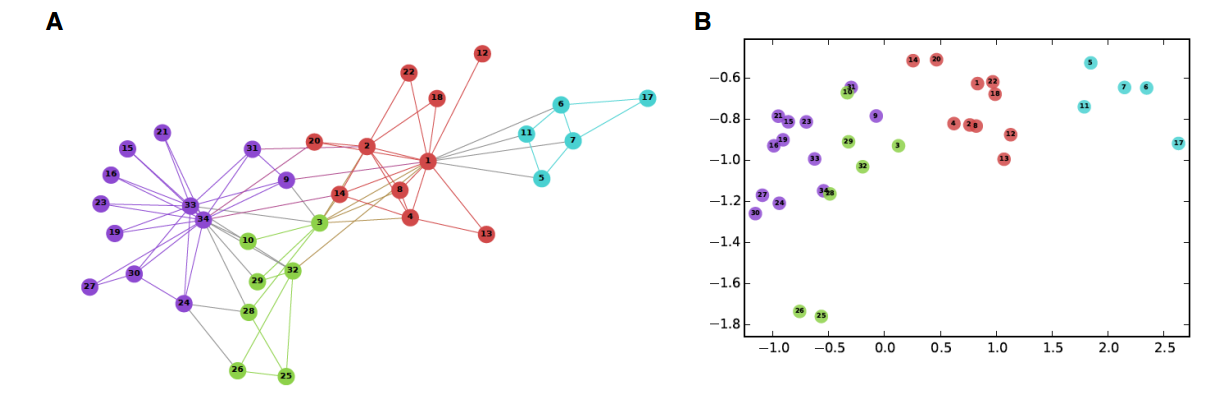
\includegraphics[width=0.65\textwidth]{figures/Node_embedding_example.png}
        \caption{\textbf A, Graph structure of the Zachary Karate Club social network, the colors represent different communities. \textbf B, Twodimensional visualization of node embeddings generated from this graph (DeepWalk method).}
        \label{fig:nodeembeddingex}
    \end{wrapfigure}
    
    The traditional approaches to learning over graphs are limited due to the fact that they \emph{require careful, hand-engineered statistics and measures}.
    
    We will introduce an alternative approach to learning over graphs: \alert{graph representation learning}. Instead of extracting hand-engineered features, we will seek to \emph{learn} representations that encode structural information about the graph.
    
\end{frame}


{\putbg
\section{An Encoder-Decoder Perspective}
}


\begin{frame}{Node embeddings}

    \begin{columns}
        \begin{column}{.45\textwidth}
        There are various methods for learning \alert{node embeddings}.
        \medskip
        
        \textbf{Goal:} encode nodes as low-dimensional vectors that summarize their graph position and the structure of their local graph neighborhood. I.e., we want to project nodes into a latent space where geometric relations correspond to relationships (e.g., edges) in the original graph.
        \medskip
        
        \textbf{Examples:} the encoder-decoder framework, factorization-based approaches, random walk embeddings.
        \end{column}
        
        \begin{column}{.55\textwidth}
        \begin{figure}[ht]
            \centering
            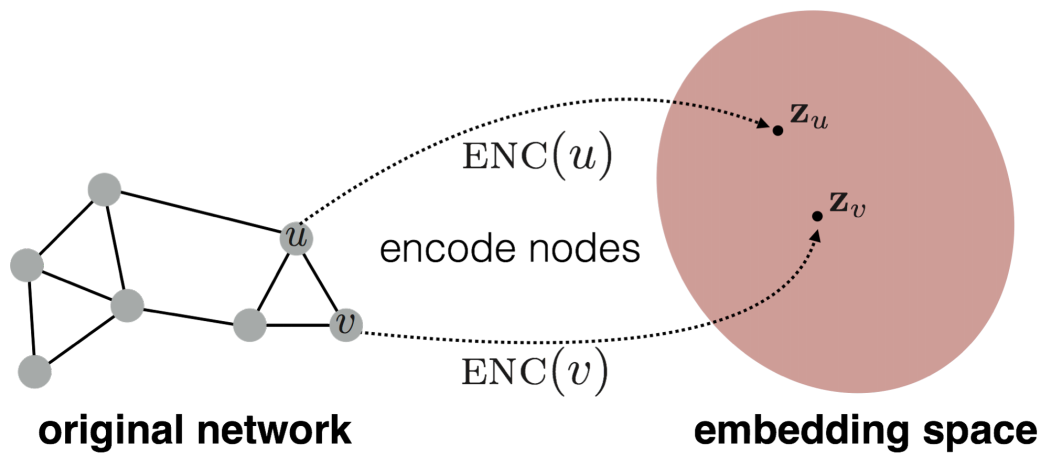
\includegraphics[width=\textwidth]{figures/Node_embedding.png}
            \caption{Illustration of the node embedding problem. Our goal is to learn an encoder (enc), which maps nodes to a low-dimensional embedding space. These embeddings are optimized so that distances in the embedding space reflect the relative positions of the nodes in the original graph.}
            \label{fig:nodeembedding}
        \end{figure}
        \end{column}
    \end{columns}
    
\end{frame}


\begin{frame}{The Encoder-Decoder Framework}

    We will focus on the framework of \alert{encoding and decoding graphs}. We view the graph representation learning problem as involving two key operations:
    \begin{itemize}
        \item[\alert{$\bullet$}] First, an \alert{encoder} model maps each node in the graph into a low-dimensional vector or embedding. 
        \item[\alert{$\bullet$}] Next, a \alert{decoder} model uses the low-dimensional node embeddings to reconstruct information about each node local neighborhood in the original graph.
    \end{itemize}

    \begin{figure}[ht]
        \centering
        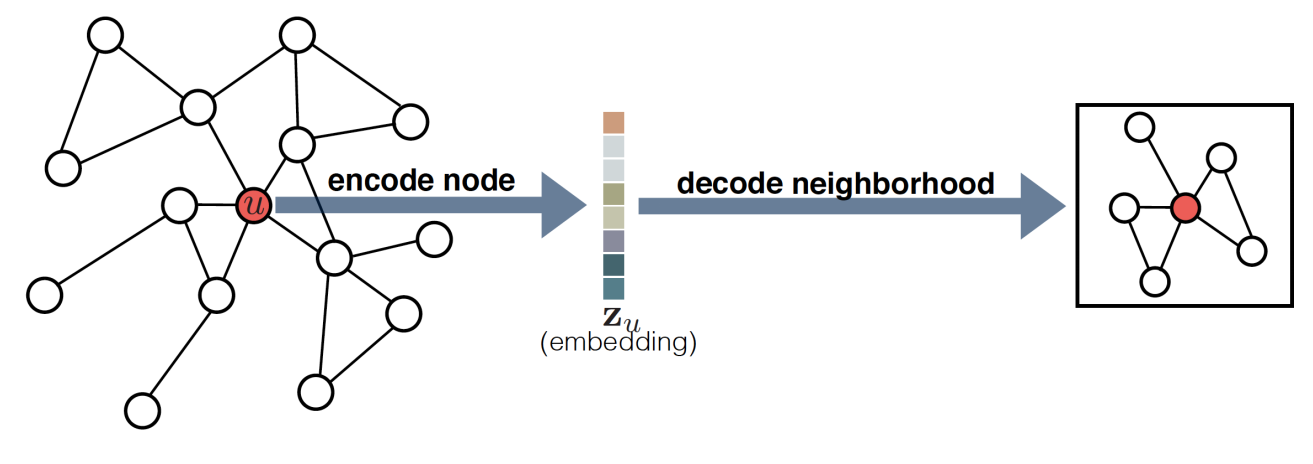
\includegraphics[height=4cm]{figures/Encoder_decoder.png}
        \label{fig:enc-dec}
    \end{figure}
    
\end{frame}


\begin{frame}{The Encoder}

    Formally, the \alert{encoder} is a function that maps nodes $v \in V$ to a corresponding \emph{vector embeddings} $\mathbf z_v \in \mathbb R^d$. In the simplest case, the encoder has the following signature:
    \begin{equation}
        \textsc{enc}: V \rightarrow \mathbb R^d,
    \end{equation}
    meaning that the encoder takes node IDs as input to generate the node embeddings.
    
    In most work on node embeddings, the encoder relies on what we call the \alert{shallow embedding} approach, where this encoder function is simply an embedding lookup based on the node ID. In other words, we have that
    \begin{equation}
        \textsc{enc}(v) = \mathbf Z[v],
        \label{eq:shallowemb}
    \end{equation}
    where $\mathbf Z \in \mathbb R^{|V| \times d}$ is a matrix containing the embedding vectors for all nodes and $\mathbf Z[v]$ denotes the row of $\mathbf Z$ corresponding to node $v$.
    
\end{frame}


\begin{frame}{The Decoder}

    The role of the \alert{decoder} is to \emph{reconstruct certain graph statistics} from the node embeddings that are generated by the encoder, e.g. predict the set of neighbors $\mathcal N(u)$ of a node $u$ or its row $\mathbf A[u]$ in the graph adjacency matrix.
    
    \alert{Pairwise decoders} are the standard and have signature: $\textsc{dec}: \mathbb R^d \times \mathbb R^d \rightarrow \mathbb R^+$.
    
    They can be interpreted as predicting the relationship or similarity between pairs of nodes, e.g. predict whether two nodes are neighbors in the graph.
    
    \textbf{Goal:} optimize the encoder and decoder to minimize the \alert{reconstruction loss} so that
    \begin{equation}
        \textsc{dec}(\textsc{enc}(u), \textsc{enc}(v)) = \textsc{dec}(\mathbf z_u, \mathbf z_v) \approx \mathbf S[u, v],
        \label{eq:reconstrloss}
    \end{equation}
    where $\mathbf S[u, v]$ is a graph-based similarity measure between nodes (e.g. \emph{neighborhood overlap statistics}). For example, the simple reconstruction objective of predicting whether two nodes are neighbors would correspond to $\mathbf S[u, v] := \mathbf A[u, v]$.
        
\end{frame}


\begin{frame}{Optimizing an Encoder-Decoder Model}

    To achieve the reconstruction objective [\Cref{eq:reconstrloss}], the standard practice is to minimize an \alert{empirical reconstruction loss} $\mathcal L$ over a set of training node pairs $\mathcal D$:
    \begin{equation}
        \mathcal L = \sum_{(u,v) \in \mathcal D} \ell (\textsc{dec}(\mathbf z_u, \mathbf z_v), \mathbf S[u, v]),
        \label{eq:loss}
    \end{equation}
    where $\ell: \mathbb R \times \mathbb R \rightarrow \mathbb R$ is a \textbf{loss function} measuring the discrepancy between the decoded (i.e., estimated) similarity values $\textsc{dec}(\mathbf z_u, \mathbf z_v)$ and the true values $\mathbf S[u, v]$.
    
    Depending on the definition of the decoder ($\textsc{dec}$) and similarity function ($\mathbf S$), the function $\ell$ might be a \textbf{mean-squared error} or even a \textbf{classification loss}, such as \emph{cross entropy}.
    
    \textbf{Objective:} \alert{train} the encoder and the decoder so that pairwise node relationships can be effectively reconstructed on the training set $\mathcal D$.
    
    Most approaches minimize the loss in \Cref{eq:loss} using \alert{stochastic gradient descent}, but there are certain instances when more specialized optimization methods (e.g., based on matrix factorization) can be used.
    
\end{frame}


\begin{frame}{Limitations of Shallow Embeddings}

    \textbf{Problems}: In shallow embedding approaches, \alert{the encoder model is simply an embedding lookup} (\Cref{eq:shallowemb}), which trains a unique embedding for each node in the graph.
    
    Besides, there are some important drawbacks:
    \begin{itemize}
        \item[\alert{$\bullet$}] They \alert{do not share any parameters} between nodes in the encoder, since the encoder directly optimizes a unique embedding vector for each node $\longrightarrow$ both statistically and computationally inefficient.
        
        \item[\alert{$\bullet$}] They \alert{do not leverage node features} in the encoder $\longrightarrow$ less informative
        
        \item[\alert{$\bullet$}] They \alert{are intrinsically \emph{transductive}}, i.e. they can only generate embeddings for nodes that were present during the training phase $\longrightarrow$ cannot be used on \emph{inductive} applications, which involve generalizing to unseen nodes after training.
    \end{itemize}

    \textbf{Solution:} use more sophisticated encoders that depend more generally on the structure and attributes of the graph $\Longrightarrow$ \alert{graph neural networks (GNNs)}.

\end{frame}


{\putbg
\section{The Graph Neural Network Model}
\label{sec:GNNmodel}
}


\begin{frame}{The simplest (and worst) GNN}

    To define a \alert{deep neural network over graphs} one could simply use the adjacency matrix as input to a deep neural network. For example, to generate an embedding of an entire graph we could simply flatten the adjacency matrix and feed the result to a multi-layer perceptron (MLP):
    \begin{equation}
        \mathbf z_G = \text{MLP}(\mathbf A[1] \oplus \mathbf A[2] \oplus \ldots \oplus \mathbf A[|\mathcal V|]);
    \end{equation}
    where $\mathbf A[i] \in \mathbf R^{|\mathcal V|}$ denotes a row of the adjacency matrix and we use $\oplus$ to denote vector concatenation.
    
    \textbf{Issue:} this approach \textit{depends on the arbitrary ordering of nodes that we used in the adjacency matrix}! In other words, such a model is \alert{\textbf{not} permutation invariant}.
    
    \begin{block}{}
    Any function $f$ that takes an adjacency matrix $\mathbf A$ as input should ideally satisfy one of the two following properties, given a permutation matrix $\mathbf P$:
    \begin{align}
        f(\mathbf{PAP}^T) = f(\mathbf A) \qquad &\text{\alert{Permutation Invariance}} \\
        f(\mathbf{PAP}^T) = \mathbf P f(\mathbf A) \qquad &\text{\alert{Permutation Equivariance}}
    \end{align}
    \end{block}
\end{frame}


\begin{frame}{Neural Message Passing}

    How we can take an input graph $G = (V, E)$, along with a set of node features $\mathbf X \in \mathbb R^{d \times |V|}$, and use this information to generate node embeddings $\mathbf z_u, \forall u \in V$?
    
    During each message-passing iteration $k$ in a GNN, a \alert{hidden embedding} $\mathbf h^{(k)}_u$ corresponding to each node $u \in V$ is updated according to information aggregated from $u$'s graph neighborhood $\mathcal N(u)$. This message-passing update can be expressed as follows:
    \begin{align}
        \mathbf h^{(k+1)}_u &= \textsc{update}^{(k)} \left( \mathbf h^{(k)}_u; \textsc{aggregate}^{(k)}(\{\mathbf h^{(k)}_v, \forall v \in \mathcal N(u)\}) \right) 
        \label{eq:mess-pass} \\
        &= \textsc{update}^{(k)} \left( \mathbf h^{(k)}_u, \mathbf m^{(k)}_{\mathcal N(u)} \right),
        \label{eq:mess-pass2}
    \end{align}
    where $\textsc{update}$ and $\textsc{aggregate}$ are arbitrary differentiable functions (i.e., \textbf{neural networks}) and $\mathbf m_{\mathcal N(u)} = \textsc{aggregate}(\{\mathbf h_v, \forall v \in \mathcal N(u)\})$ is the ``message'' that is aggregated from $u$'s graph neighborhood $\mathcal N(u)$ (\alert{neighborhood aggregation operation}). The different iterations of message passing are also sometimes known as the different ``layers'' of the GNN.

\end{frame}


\begin{frame}{Message Passing in Practice}

    The initial embeddings at $k = 0$ are set to the input features for all the nodes, i.e., $\mathbf h^{(0)}_u = \mathbf x_u, \forall u \in \mathcal V$. After running $K$ iterations of the GNN message passing, we can use the \textbf{output of the final layer} to define the \alert{embeddings} for each node, i.e.,
    \begin{equation}
        \mathbf z_u = \mathbf h^{(K)}_u, \forall u \in \mathcal V.
    \end{equation}
    Since $\textsc{aggregate}$ takes a set as input, GNNs are \alert{permutation equivariant} by design!
    
    \textbf{Basic intuition} $\longrightarrow$ at each iteration, every node aggregates information from its local neighborhood, and as these iterations progress each node embedding contains more and more information from further reaches of the graph.
    
    \begin{itemize}
        \item[\alert{$\bullet$}] \emph{structural information} about the graph $\longrightarrow$ after $k$ iterations, $\mathbf h^{(k)}_u$ might encode information about the \alert{degrees} of all the nodes in $u$'s $k$-hop neighborhood.
    
        \item[\alert{$\bullet$}] \emph{feature-based information} about the graph $\longrightarrow$ after $k$ iterations, $\mathbf h^{(k)}_u$ also encodes information about all the \alert{features} in its $k$-hop neighborhood $\rightarrow$ analogous to convolutional kernels in CNNs!
    \end{itemize}
    
\end{frame}


\begin{frame}{The Basic GNN}

    The basic GNN message passing is defined as
    \begin{equation}
        \mathbf h^{(k)}_u = \sigma \left( \mathbf W^{(k)}_\text{self} \; \mathbf h_u^{(k-1)} + \mathbf W_\text{neigh}^{(k)} \sum_{v \in \mathcal N(u)} \mathbf h^{(k-1)}_v + \mathbf b^{(k)} \right),
    \end{equation}
    where $\mathbf W^{(k)}_\text{self}, \mathbf W_\text{neigh}^{(k)} \in \mathbb R^{d^{(k)} \times d^{(k-1)}}$ are \alert{trainable parameter matrices} and $\sigma$ denotes an \alert{elementwise non-linearity} (e.g., a tanh or ReLU). The \alert{bias term} $b^{(k)} \in \mathbb R^{d^{(k)}}$ is often omitted for notational simplicity, but including it can be important to achieve strong performance.
    
    We can equivalently define the basic GNN through the \textsc{update} and \textsc{aggregate} functions:
    \begin{align}
        &\mathbf m_{\mathcal N(u)} = \sum_{v \in \mathcal N(u)} \mathbf h_v, 
        \label{eq:basicgnn} \\
        &\textsc{update}(\mathbf h_u, \mathbf m_{\mathcal N(u)}) = \sigma \left( \mathbf W_\text{self} \; \mathbf h_u + \mathbf W_\text{neigh} \; \mathbf m_{\mathcal N(u)} \right),
    \end{align}
    
\end{frame}

\begin{frame}{f}
    
    Any GNNs can also be succinctly defined using graph-level equations. In the case of a basic GNN, we can write the graph-level definition of the model as follows:
    \begin{equation}
        \mathbf H^{(k)} = \sigma \left( \mathbf{A H}^{(k-1)} \mathbf W_\text{neigh}^{(k)} + \mathbf H^{(k-1)} \mathbf W_\text{self}^{(k)} \right),
    \end{equation}
    where $\mathbf H^{(k)} \in \mathbb R^{|V| \times d}$ denotes the matrix of node representations at layer $k$ in the GNN (with each node corresponding to a row in the matrix), $\mathbf A$ is the graph adjacency matrix, and we have omitted the bias term for notational simplicity.
    
    \begin{figure}
        \begin{minipage}{0.49\textwidth}
            \caption{Overview of encoding in the neighborhood aggregation methods.
            To generate an embedding for node \texttt{A}, the model aggregates messages from \texttt{A}'s local graph neighbors (\textit{i.e.}, \texttt{B}, \texttt{C}, and \texttt{D}), and in turn, the messages coming from these neighbors are based on information aggregated from their respective neighborhoods, and so on.
            A ``depth-2'' version of this idea is shown (\textit{i.e.}, information is aggregated from a two-hop neighborhood around node \texttt{A}), but in principle these methods can be of an arbitrary depth.
            %At the final ``depth'' or ``layer'' the initial messages are based on the input node attributes.
            % Overview of how a single node aggregates messages from its local neighborhood. The model aggregates messages from \texttt{A}'s local graph neighbors (\textit{i.e.}, \texttt{B}, \texttt{C}, and \texttt{D}), and in turn, the messages coming from these neighbors are based on information aggregated from their respective neighborhoods, and so on. This visualization shows a two-layer version of a message-passing model. Notice that the computation graph of the GNN forms a tree structure by unfolding the neighborhood around the target node.
        }
        \end{minipage}
        \begin{minipage}[b]{0.49\textwidth}
            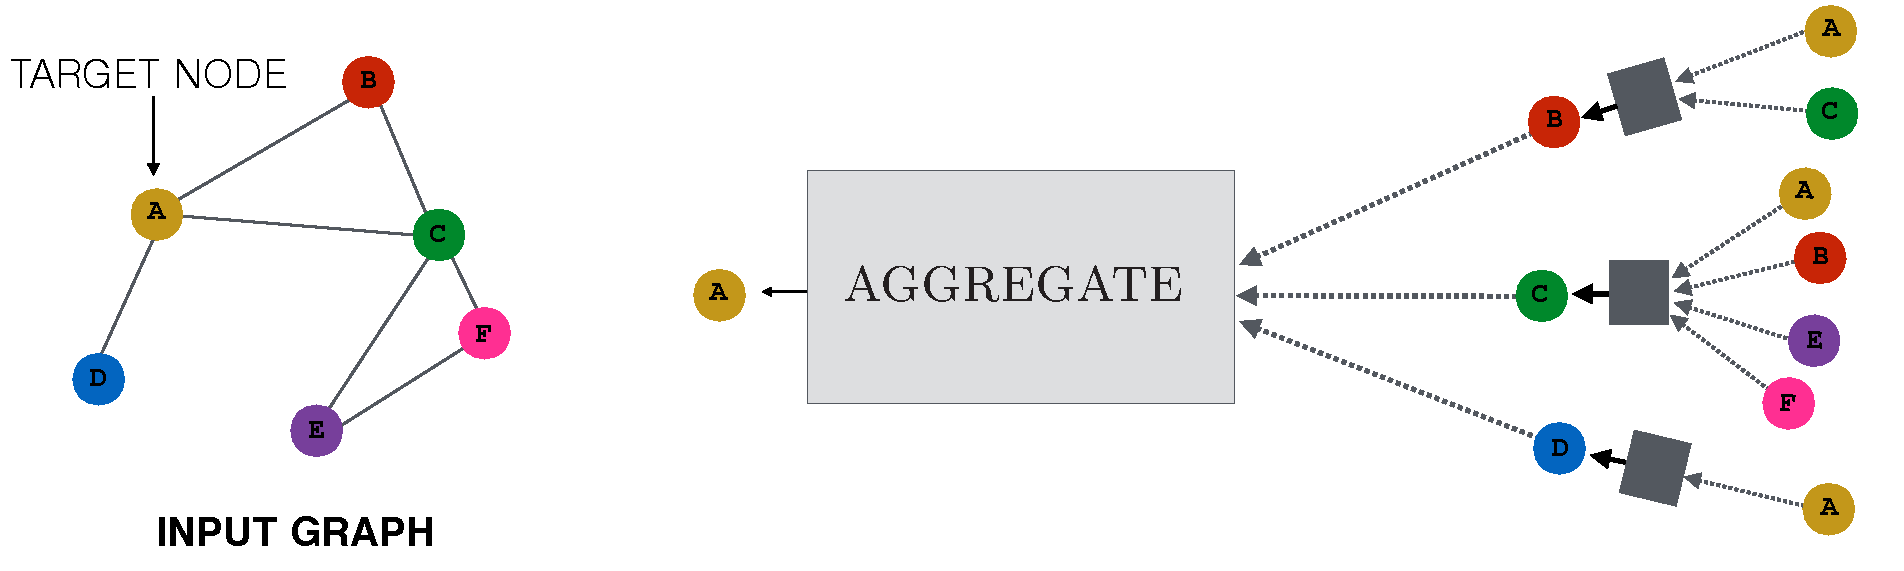
\includegraphics[width=1.1\textwidth]{neigh_agg_new.pdf}
        \end{minipage}
        \label{fig:neigh_agg}
    \end{figure}
    
\end{frame}


\begin{frame}{Message Passing with Self-loops}

    As a simplification of the neural message passing approach, it is common to \emph{add self-loops to the input graph and omit the explicit update step} $\longrightarrow$ \alert{self-loop approach}
    \medskip
    
    We define the message passing simply as
    \begin{equation}
        \mathbf h^{(k)}_u = \textsc{aggregate}(\{\mathbf h_v^{(k-1)}, \; \forall v \in \mathcal N(u) \cup \{u\}\}),
    \end{equation}
    where now the aggregation is taken over the set $\mathcal N(u) \cup \{u\}$, i.e., \emph{the node's neighbors as well as the node itself} $\longrightarrow$ we no longer need to define an explicit update function, as the update is implicitly defined through the aggregation method.
    \medskip
    
    In the case of the basic GNN, adding self-loops is equivalent to  sharing parameters between the $\mathbf W_\text{self}$ and $\mathbf W_\text{neigh}$ matrices, which gives the following \alert{graph-level update}:
    \begin{equation}
        \mathbf H^{(k)} = \sigma \left( (\mathbf A + \mathbf I) \mathbf H^{(k-1)} \mathbf W^{(k)} \right) .
    \end{equation}
    
    \textbf{Benefits:} no longer need to define an explicit update function and this simplification \alert{alleviates overfitting}, but it also severely \alert{limits the expressivity} of the GNN
    %as the information coming from the node's neighbours cannot be differentiated from the information from the node itself.

\end{frame}


\begin{frame}{Graph convolutional networks (GCNs)}

    \textbf{Issue with the basic neighborhood aggregation operation [\Cref{eq:basicgnn}]:} it can be \alert{unstable} and \alert{highly sensitive to node degrees}.
    
    \textbf{Solution:} \emph{normalize the aggregation operation} using the degrees of the nodes involved:
    \begin{equation}
        \mathbf m_{\mathcal N(u)} = \frac{\sum_{v \in \mathcal N(u)} \mathbf h_v}{|\mathcal N(u)|}.
    \end{equation}
    
    Another normalization factor is the \alert{symmetric normalization}:
    \begin{equation}
        \mathbf m_{\mathcal N(u)} = \sum_{v \in \mathcal N(u)} \frac{\mathbf h_v}{\sqrt{|\mathcal N(u)| |\mathcal N(v)|}}.
    \end{equation}
    
    The popular \alert{graph convolutional network (GCN)} employs the \emph{symmetric-normalized aggregation} as well as the \emph{self-loop approach}, using as message passing function
    \begin{equation}
        h^{(k)}_u = \sigma \left( \mathbf W^{(k)} \sum_{v \in \mathcal N(u) \cup \{u\}} \frac{\mathbf h_v}{\sqrt{|\mathcal N(u)| |\mathcal N(v)|}} \right).
    \end{equation}

\end{frame}


\begin{frame}{Improving the Aggregation Layer}

    An aggregation function with the following form is a \alert{universal set function approximator}:
    \begin{equation}
        \mathbf m_{\mathcal N(u)} = \textbf{MLP}_\theta \left( \sum_{v \in \mathcal N(u)} \textbf{MLP}_\phi (\mathbf h_v) \right).
        \label{eq:univsetapproxf}
    \end{equation}
    So any permutation-invariant function that maps a set of embeddings to a single embedding can be approximated to an arbitrary accuracy by a model using \Cref{eq:univsetapproxf}.\\
    $\longrightarrow$ \alert{set pooling} leads small increases in performance but increased risk of overfitting
    
    Another strategy is to apply \alert{attention}: assign an attention weight or importance to each neighbor, which is used to weigh this neighbor's influence during the aggregation step. The first GNN model to apply this style of attention was the \alert{Graph Attention Network (GAT)}:
    \begin{equation}
        \mathbf m_{\mathcal N(u)} = \sum_{v \in \mathcal N(u)} \alpha_{u,v} \mathbf h_v,
    \end{equation}
    where $\alpha_{u,v}$ denotes the attention on neighbor $v \in \mathcal N(u)$ (\emph{neighborhood attention}) when we are aggregating information at node $u$.
    
\end{frame}


\begin{frame}{Visualize a single GAT step}

    \begin{columns}[onlytextwidth]
        \begin{column}{.5\textwidth}
            \begin{figure}
                \centering
                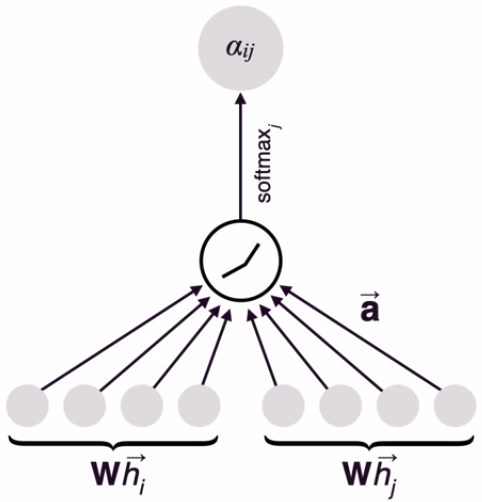
\includegraphics[width=0.65\textwidth]{figures/GAT_step_1.png}
                \caption{Attention mechanism. It looks at features of node $i$ and its neighbor $j$, then the attention function computes the coefficient $\alpha_{ij}$, which signifies the influence of node $i$ to node $j$.}
                \label{fig:GAT_step_1}
            \end{figure}
        \end{column}
        
        \begin{column}{.5\textwidth}
            \begin{figure}
                \centering
                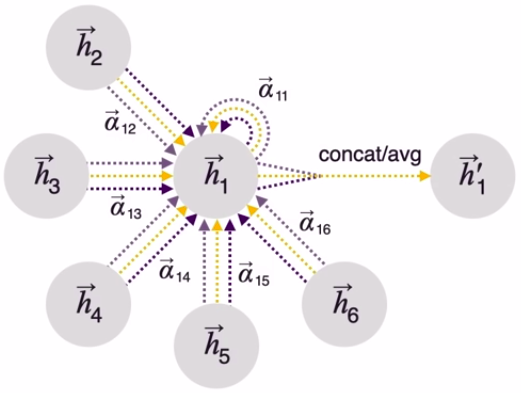
\includegraphics[width=0.8\textwidth]{figures/GAT_step_2.png}
                \caption{Multi-head attention mechanism. Each colored line indicates a different way in which the node receives information from its immediate neighbors, which is aggregated to produce an updated representation.}
                \label{fig:GAT_step_2}
            \end{figure}
        \end{column}
    \end{columns}
    \footnotesize{Images from \cite{PetarIntroGNN}}
\end{frame}


\begin{frame}{Graph Pooling}

    What if we want to learn an embedding $\mathbf z_G$ for the entire graph $G$? $\longrightarrow$ \alert{graph pooling}
    
    We want to design a pooling function $f_p$, which maps a set of node embeddings $\{\mathbf z_1, \ldots, \mathbf z_{|V|} \}$ to an embedding $\mathbf z_G$ that represents the full graph.
    
    One approach is to simply to take a sum (or mean) of the node embeddings:
    \begin{equation}
        \mathbf z_G = \frac{\sum_{v \in V} \mathbf z_u}{f_n(|V|)},
    \end{equation}
    where $f_n$ is some normalizing function e.g., the identity function, so
    \begin{equation}
        \mathbf z_G = \frac{\sum_{v \in V} \mathbf z_u)}{|V|}.
    \end{equation}
    \textbf{Limitation}: it does not exploit the structure of the graph! We want to exploit the graph topology at the pooling stage $\longrightarrow$ use \alert{graph clustering or coarsening}
    
\end{frame}


\begin{frame}{Generalized Message Passing}
    
    The GNN message passing approach can also be generalized to leverage edge and graph-level information at each stage of message passing, instead of operating only at the node level. 
    
    In \cite{battaglia2018relational} we can find a \alert{more general approach}: we define each iteration of message passing according to the equations (\textbf{which we revised})
    \begin{align}
        \mathbf h^{(k)}_{(u,v)} &= \textsc{update}_\text{edge} \left( \mathbf h_{(u,v)}^{(k-1)}, \mathbf h_u^{(k-1)}, \mathbf h_v^{(k-1)}, \mathbf h_G^{(k-1)} \right) \qquad &\forall (u,v) \in E \qquad
        \label{eq:upedge} \\
        \mathbf m_{\mathcal N(u)}^{(k)} &= \textsc{aggregate}_{e \to v} \left( \left\{ \mathbf h_{(u,v)}^{(k)}, \; \forall v \in \mathcal N(u) \right\} \right) \qquad &\forall u \in V \qquad
        \label{eq:message} \\
        \mathbf h^{(k)}_u &= \textsc{update}_\text{node} \left( \mathbf h_u^{(k-1)}, \mathbf m_{\mathcal N(u)}, \mathbf h_G^{(k-1)} \right) \qquad &\forall u \in V \qquad
        \label{eq:upnode} \\
        \mathbf m_{e}^{(k)} &= \textsc{aggregate}_{e \to G} \left( \left\{ \mathbf h_{(u,v)}^{(k)}, \forall (u, v) \in E \right\} \right)
        \label{eq:aggeG} \\
        \mathbf m_{v}^{(k)} &= \textsc{aggregate}_{v \to G} \left( \left\{ \mathbf h_u^{(k)}, \, \forall u \in V \right\} \right)
        \label{eq:aggvG} \\
        \mathbf h^{(k)}_G &= \textsc{update}_\text{graph} \left(\mathbf h_G^{( k-1)}, \mathbf m_{v}^{(k)}, \mathbf m_{e}^{(k)} \right).
        \label{eq:upgraph}
    \end{align}
\end{frame}


\begin{frame}{Generalized Message Passing Innovation}

    The important innovation in this generalized message passing framework is that, during message passing, we generate:
    \begin{itemize}
    \item[\alert{$\bullet$}] a hidden embedding $\mathbf h^{(k)}_u$ corresponding to \alert{each node} $u \in V$ in the graph,
    \item[\alert{$\bullet$}] a hidden embeddings $\mathbf h_{(u,v)}^{(k)}$ for \alert{each edge} $(u, v) \in E$ in the graph,
    \item[\alert{$\bullet$}] an embedding $\mathbf h_G^{(k)}$ corresponding to the \alert{entire graph} $G$.
    \end{itemize}
    
    This allows the message passing model to \textbf{easily integrate edge and graph-level features}, and recent work has also shown this generalized message passing approach to have benefits compared to a standard GNN in terms of \textbf{logical expressiveness}. Generating embeddings for edges and the entire graph during message passing also makes it \textbf{trivial to define loss functions} based on graph or edge-level classification tasks.
    
\end{frame}


\begin{frame}{}
    
    \begin{minipage}{\textwidth}
    \begin{algorithm}[H]
        \begin{algorithmic}
        \Function{GraphNetwork}{$\{ \mathbf h_{(u,v)}^{(k-1)}, \forall (u, v) \in E\}$, $\{ \mathbf h_u^{(k-1)}, \, \forall u \in V\}$, $h_G^{(k-1)}$}
            \For {$(u, v) \in |E|$}
                \State $\mathbf h^{(k)}_{(u,v)} \gets \textsc{update}_\text{edge} (\mathbf h_{(u,v)}^{(k-1)}, \mathbf h_u^{(k-1)}, \mathbf h_v^{(k-1)}, \mathbf h_G^{(k-1)})$
                \Comment{1. Compute updated edge attributes}
            \EndFor
            \For {$u \in |V|$}
                \State $\mathbf m_{\mathcal N(u)}^{(k)} \gets \textsc{aggregate}_{e \to v}(\{ \mathbf h_{(u,v)}^{(k)}, \; \forall v \in \mathcal N(u) \})$
                \Comment{2. Aggregate edge attributes per node}
                \State $\mathbf h^{(k)}_u \gets \textsc{update}_\text{node} ( \mathbf h_u^{(k-1)}, \mathbf m_{\mathcal N(u)}, \mathbf h_G^{(k-1)})$
                \Comment{3. Compute updated node attributes}
            \EndFor
            \State $\textbf m_{e}^{(k)} \gets \textsc{aggregate}_{e \to G} \left( \{ \mathbf h_{(u,v)}^{(k)}, \forall (u, v) \in E\} \right)$
            \Comment{4. Aggregate edge attributes globally}
            \State $\textbf m_{v}^{(k)} \gets \textsc{aggregate}_{v \to G} \left( \{ \mathbf h_u^{(k)}, \, \forall u \in V\} \right)$
            \Comment{5. Aggregate node attributes globally}
            \State $\mathbf h^{(k)}_G \gets \textsc{update}_\text{graph}(\mathbf h_G^{( k-1)}, \textbf m_{v}^{(k)}, \textbf m_{e}^{(k)})$
            \Comment{6. Compute updated global attribute}
            \State \Return $\{ \mathbf h_{(u,v)}^{(k)}, \forall (u, v) \in E\}$, $\{ \mathbf h_u^{(k)}, \, \forall u \in V\}$, $h_G^{(k-1)}$
        \EndFunction
        \end{algorithmic}
        \caption{Steps of computation in a GNN layer.}
        \label{alg:gn}
    \end{algorithm}
    \end{minipage}
    
\end{frame}


\begin{frame}[allowframebreaks]{Graph Neural Networks in Practice}
%GNN real-world applications

    In the vast majority of current real-world applications, GNNs are used for:
    \begin{itemize}
        \item[\alert{$\bullet$}] \emph{Node Classification} $\rightarrow$ train GNNs in a fully-supervised manner with a negative log-likelihood loss:
        \begin{equation}
            \mathcal L = \sum_{u \in V_\text{train}} -\log(\text{softmax}(\mathbf z_u, \mathbf y_u))
            \label{eq:lossnodeclass}
        \end{equation}
        where $\mathbf y_u$ is a one-hot vector indicating the class of training node $u \in V_\text{train}$ and we use $\text{softmax}(\mathbf z_u, \mathbf y_u)$ to denote the predicted probability that the node belongs to the class $\mathbf y_u$, computed via the $\text{softmax}$ function:
        \begin{equation}
            \text{softmax}(\mathbf z_u, \mathbf y_u) = \sum^c_{i=1} \mathbf y_u[i] \frac{e^{\mathbf z_u^\top \mathbf w_i}}{\sum^c_{j=1} e^{\mathbf z_u^\top \mathbf w_j}},
        \end{equation}
        where $\mathbf w_i \in \mathbb R^d, i = 1, \ldots, c$ are trainable parameters.
        
        \item[\alert{$\bullet$}] \emph{Graph Classification} $\rightarrow$ use a softmax classification loss --- analogous to \Cref{eq:lossnodeclass} --- with the key difference that the loss is computed with graph-level embeddings $\mathbf z_{G_i}$ over a set of labeled training graphs $\mathcal G = \{G_1, \ldots, G_n\}$.
        
        \item[\alert{$\bullet$}] \emph{Graph Regression} $\rightarrow$ employ a squared-error loss of the following form:
        \begin{equation}
            \mathcal L = \sum_{G_i \in \mathcal G} \| \textbf{MLP}(\mathbf z_{G_i}) - y_{G_i}\|_2^2,
        \end{equation}
        where $\textbf{MLP}$ is a densely connected neural network with a univariate output and $y_{G_i} \in \mathbb R$ is the target value for training graph $G_i$.
        
        \item[\alert{$\bullet$}] \emph{Edge Prediction} $\rightarrow$ employ the pairwise node embedding loss functions. In principle, GNNs can be combined with any pairwise loss function, with the output of the GNNs replacing the shallow embeddings.
    \end{itemize}
\end{frame}


{\putbg
\section{Combinatorial Optimization and Reasoning with GNN}}


\begin{frame}{Relational Inductive Biases in GNN - \cite{battaglia2018relational}}

    \begin{block}{}
        \alert{Relational inductive biases} are inductive biases\footnote{An inductive bias allows a learning algorithm to prioritize one solution (or interpretation) over another, independent of the observed data. E.g., in a Bayesian model it is the choice and parameterization of the prior.} which impose constraints on relationships and interactions among entities in a learning process.
    \end{block}

    \begin{itemize}
        \item[\alert{$\bullet$}] Graphs can express arbitrary relationships among entities, which means the GNN's input determines how \alert{entities interact or are isolated} via the edges, rather than those choices being determined by the fixed architecture.
        
        \item[\alert{$\bullet$}] Graphs represent entities and their relations as sets, which are invariant to permutations. This means GNNs are \alert{invariant to the order} of these elements, which is often desirable.
        
        \item[\alert{$\bullet$}] A GNN's $\textsc{update}_\text{edge}$ and $\textsc{update}_\text{node}$ functions are reused for all edges and nodes. This means GNNs automatically support a form of \alert{combinatorial generalization}: a single GNN can operate on graphs of different sizes (numbers of edges and nodes) and shapes (edge connectivity).
    \end{itemize}
    
\end{frame}


\begin{frame}{Frame Title - \cite{cappart2021combinatorial}}

    The inductive bias of GNNs effectively encodes combinatorial and relational input due to their invariance to permutations and awareness of input sparsity.
    
    Intuitively, CO deals with problems that involve optimizing a cost (or objective) function by selecting a subset from a finite set, with the latter encoding constraints on the solution space.
    
    Beyond using standard GNN models for CO, the emerging paradigm of algorithmic reasoning provides new perspectives on designing and training GNNs that satisfy natural invariants and properties, enabling improved generalization and interpretability.
    
    Neural networks are traditionally powerful in the interpolation regime, i.e., when we expect the distribution of unseen (``test'') inputs to roughly match the distribution of the inputs used to train the network. However, they tend to struggle when extrapolating, i.e., when they are evaluated out-of-distribution. For example, merely increasing the test input size, e.g., the number of nodes in the input graph, is often sufficient to lose most of the training's predictive power. Extrapolating is a potentially important issue for tackling CO problems with (G)NNs trained end-to-end. As a critical feature of a powerful reasoning system, it should apply to any plausible input, not just ones within the training distribution. Therefore, unless we can accurately foreshadow the kinds of inputs our neural CO approach will be solving, it could be essential to address the issue of out-of-distribution generalization in neural networks meaningfully.
    
\end{frame}


{\putbgdark
\begin{frame}[standout]
	\begin{center}
		\Large \uncover<+->{Thank you for your attention!}
		
		\Huge\uncover<+->{\Smiley}
	\end{center}
\end{frame}
}

\begin{frame}[allowframebreaks, noframenumbering, plain]{}

	\nocite{*}
	\printbibliography

\end{frame}

\end{document}